\documentclass[a4paper]{article}




\usepackage[margin=1in]{geometry} % full-width

% AMS Packages
\usepackage{amsmath}
\usepackage{amsthm}
\usepackage{amssymb}

% Unicode
\usepackage[utf8]{inputenc}
\usepackage{hyperref}
\hypersetup{
	unicode,
%	colorlinks,
%	breaklinks,
%	urlcolor=cyan, 
%	linkcolor=blue, 
	pdfauthor={Author One, Author Two, Author Three},
	pdftitle={A simple article template},
	pdfsubject={A simple article template},
	pdfkeywords={article, template, simple},
	pdfproducer={LaTeX},
	pdfcreator={pdflatex}
}

% Vietnamese
%\usepackage{vntex}

% Natbib 


\usepackage[sort&compress,numbers,square]{natbib}
\bibliographystyle{mplainnat}

% Theorem, Lemma, etc
\theoremstyle{plain}
\newtheorem{theorem}{Theorem}
\newtheorem{corollary}[theorem]{Corollary}
\newtheorem{lemma}[theorem]{Lemma}
\newtheorem{claim}{Claim}[theorem]
\newtheorem{axiom}[theorem]{Axiom}
\newtheorem{conjecture}[theorem]{Conjecture}
\newtheorem{fact}[theorem]{Fact}
\newtheorem{hypothesis}[theorem]{Hypothesis}
\newtheorem{assumption}[theorem]{Assumption}
\newtheorem{proposition}[theorem]{Proposition}
\newtheorem{criterion}[theorem]{Criterion}
\theoremstyle{definition}
\newtheorem{definition}[theorem]{Definition}
\newtheorem{example}[theorem]{Example}
\newtheorem{remark}[theorem]{Remark}
\newtheorem{problem}[theorem]{Problem}
\newtheorem{principle}[theorem]{Principle}

\usepackage{graphicx, color}
\graphicspath{{fig/}}

%\usepackage[linesnumbered,ruled,vlined,commentsnumbered]{algorithm2e} % use algorithm2e for typesetting algorithms
\usepackage{algorithm, algpseudocode} % use algorithm and algorithmicx for typesetting algorithms
\usepackage{mathrsfs} % for \mathscr command



% Author info

\begin{document}
    \begin{titlepage}
        \centering
        {
\includegraphics[width=0.2\textwidth]{logo}\par}
        \vspace{1cm}
        {\bfseries\LARGE Universidad Castilla La Mancha \par}
        \vspace{1cm}
        {\scshape\Large Ingeniería informática \par}
        \vspace{3cm}
        {\scshape\Huge linear data structure \par}
        \vspace{3cm}
        {\itshape\Large Data Structure laboratory\par}
        \vfill
        {\Large Authors: \par}
        {\Large  Juan Gigante Rios\par Andrés González Varela  \par  María Jesús Dueñas Recuero }
        \vfill
        {\Large 11th November 2021 \par}
    \end{titlepage}
	

\newpage
	\tableofcontents
	\newpage
	\section{Stack}
        \subsection{Problem description}
        There is a data file containing natural numbers. This file will be read number by number and you must apply the following treatment:
        \begin{itemize}
            \item Place the first number on a first stack.
            \item The following numbers will be compared with the one on top of the first stack. When the addition of the read number with the number on top is nine, you must insert two times the lower of the two on a second stack and remove the number on top of the first stack.
            \item If the addition is not nine, the read number must be placed on the first stack. Once finished the first treatment, you must empty the second stack number by number in a way that, when two or more consecutive numbers add up to nine or more, a nine must be placed on a third stack.
        \end{itemize}
        The final output of the program will be the number of nines contained in the third stack.

     \subsection{Approach}
        The main idea to develop this project is to divide it into classes according to each of the functions. That is why, we have created a \textbf{ReadFile} class which is in charge of reading the file provided to us for the practice, the \textbf{Problem} class where most of the code will be developed solving the problem and finally, the \textbf{Main} class where only calls to methods of the classes will be made and the result will be shown by console. All this by means of an object oriented programming.


        \subsubsection{ReadFile class}
        \begin{itemize}
            \item \textbf{read-File}\par
            In order to read the file given to us, and taking into account that the practices consist in the use and handling of stacks, we have considered storing the information of this file in a stack,\textbf{aux-number-Stack-file }.

             As when storing it in a stack the information will be stored inversely to how we read it, we use another stack ,\textbf{number-Stack-File}, to re-invert the information and make it look as it is read in the file so that it is easier to work with.Therefore, this method will return a stack with the information from the file figure[1].\newline
             \item \textbf{Read-file constructor}\par
           The constructor method is a special method to create and initialise an object created from a class, in our case to create an object of the class "ReadFile".
        \end{itemize}
        
             \begin{figure}[h]
                \centering
                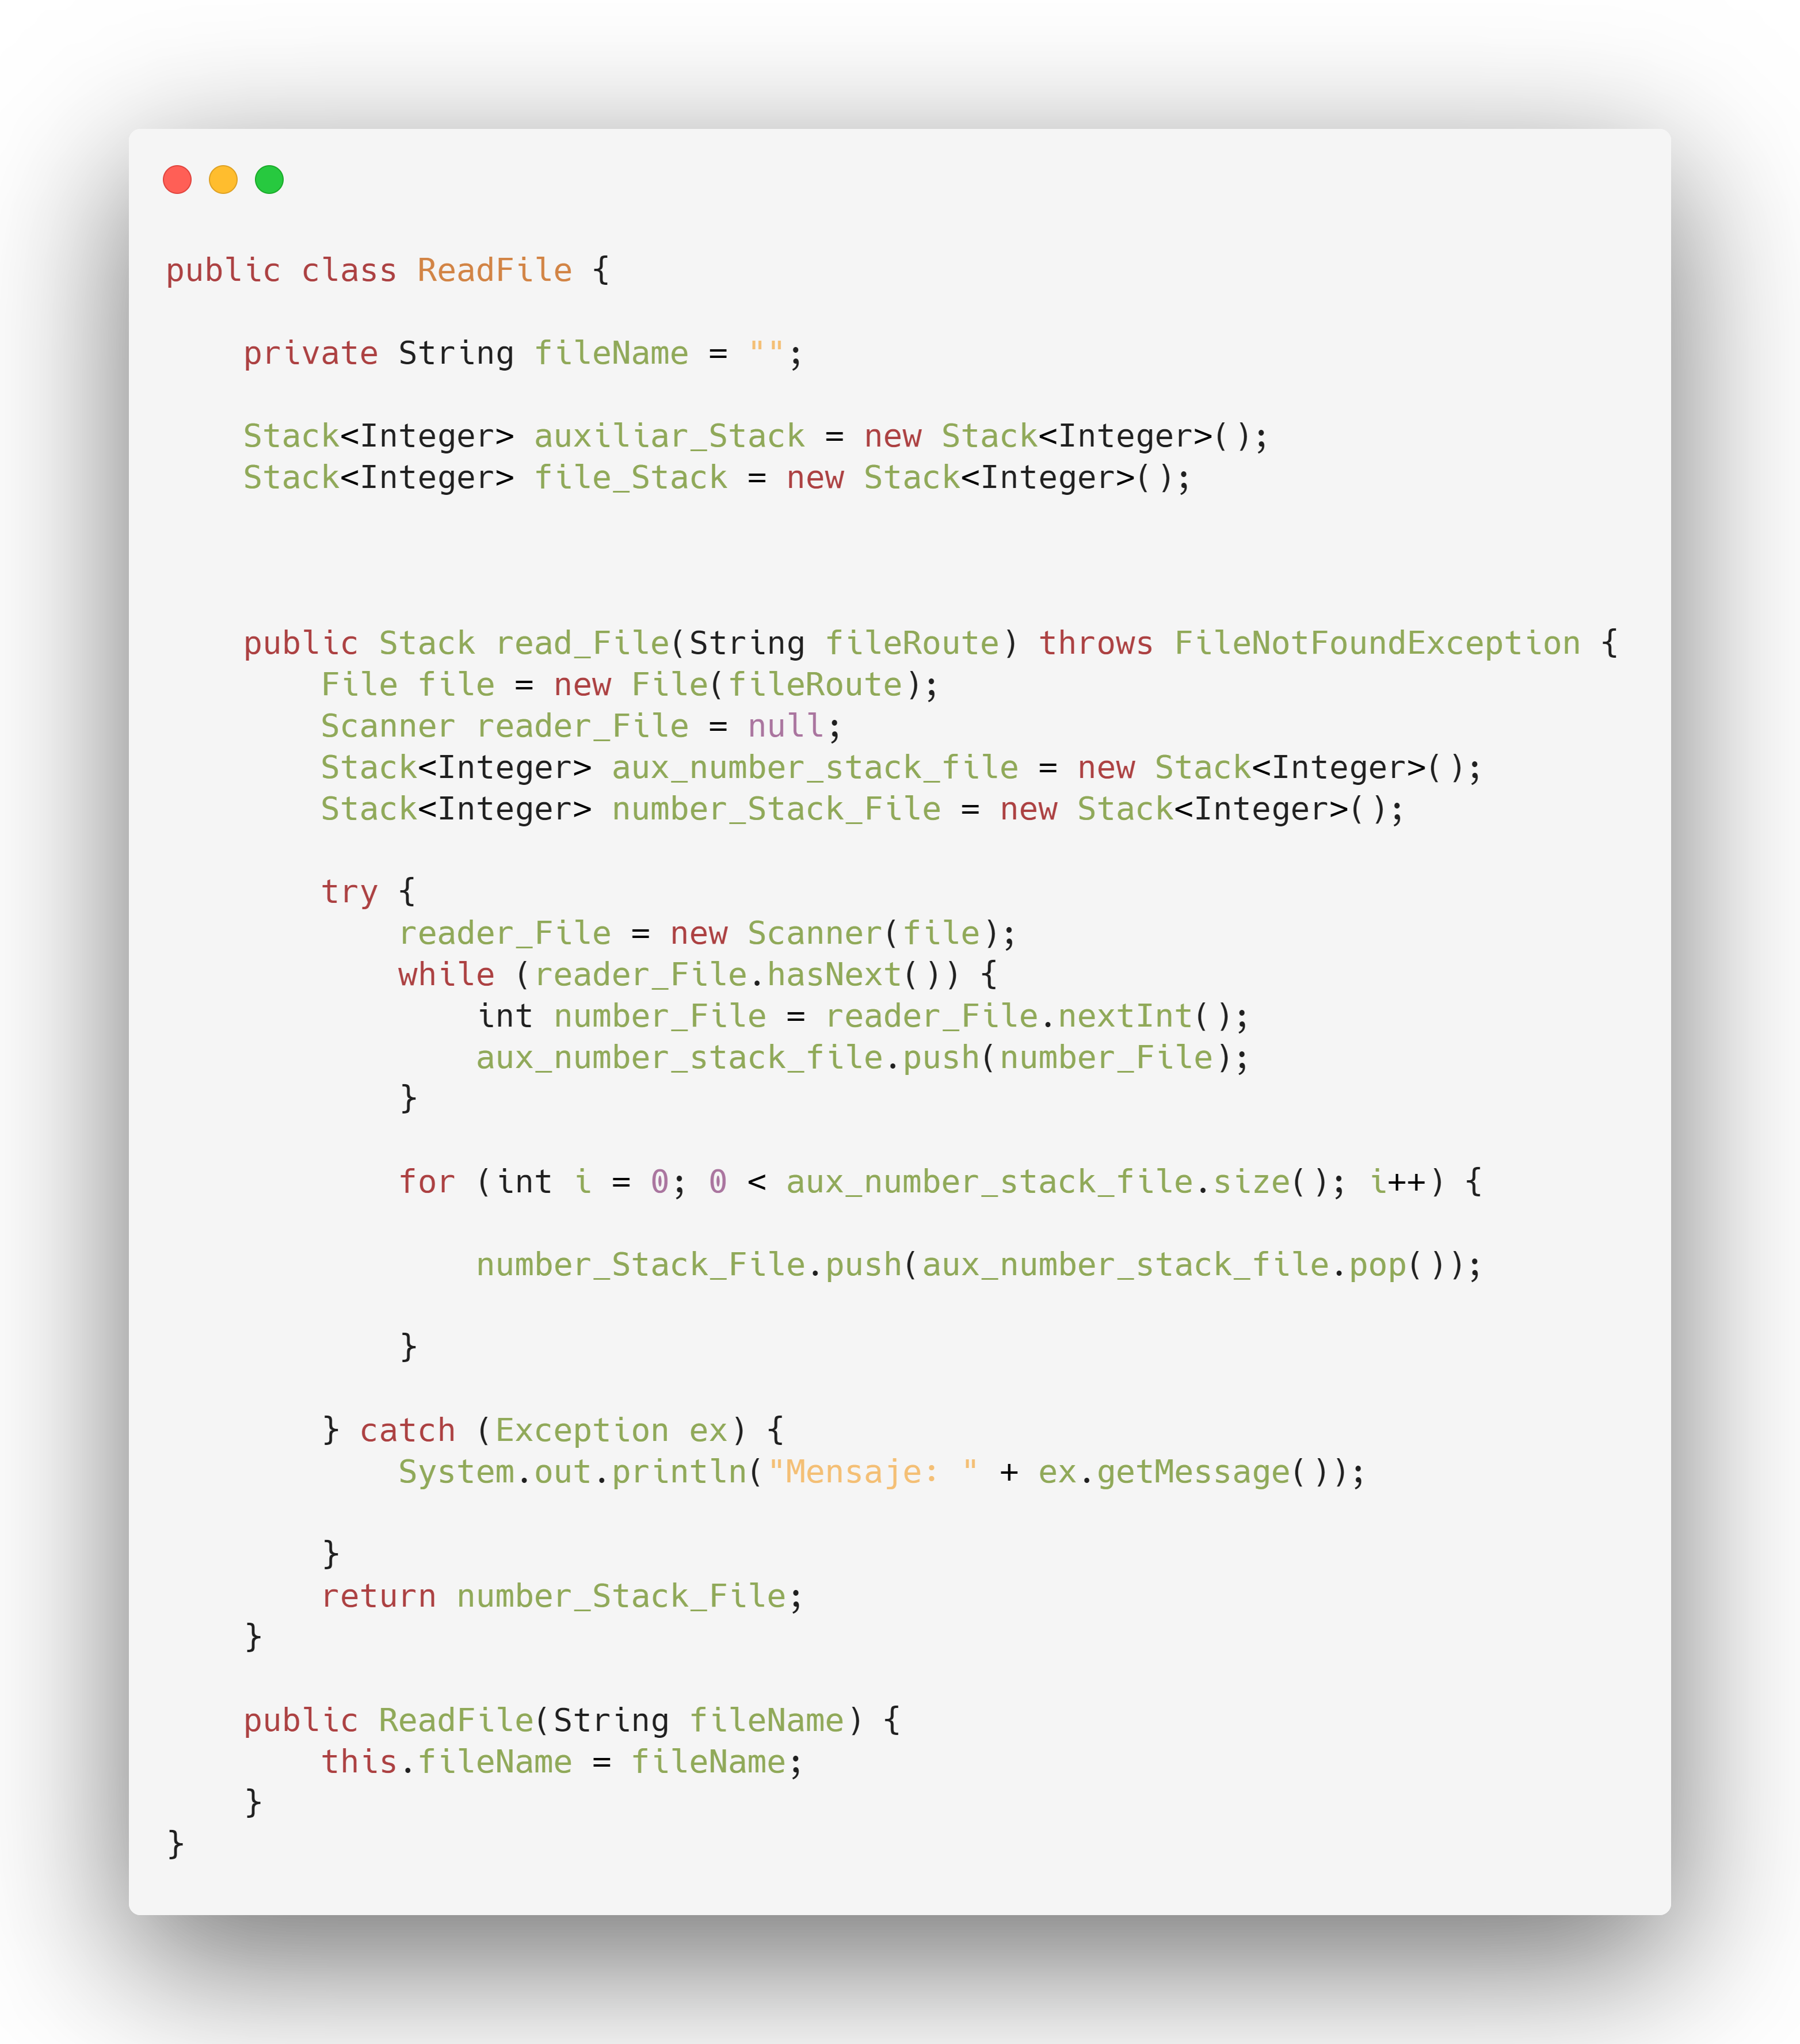
\includegraphics[width=300pt\textwidth]{read-file.png}
                \caption{Code of the ReadFile class}
                \label{fig:mesh1}
            \end{figure}
        

\newpage
        \subsubsection{Problem class}
            \begin{itemize}
                \item \textbf{fill-Stacks}
                This method is the body of the class, it is where we try to solve the practice. The main idea of this method is to read the file-stack (containing the numbers to be read) where the first number of this file is put into the first-stack and the last top number in this row is added to the file-stack.\par

                Afterwards, if the sum is nine, the smallest sum will be added to the second-stack, otherwise it will return to the first-stack.\par

                We use the FileNotFoundException and EmptyStackException exceptions to control that the file is found and that if the stack is empty it does not crash the program, respectively.\par

                As an important clarification we have used the condition if(i==0) in line 28, to control that only one file-stack number is inserted in each iteration since it was giving us problems if we didn't control it.\par
                \begin{figure}[h]
                     \centering
                     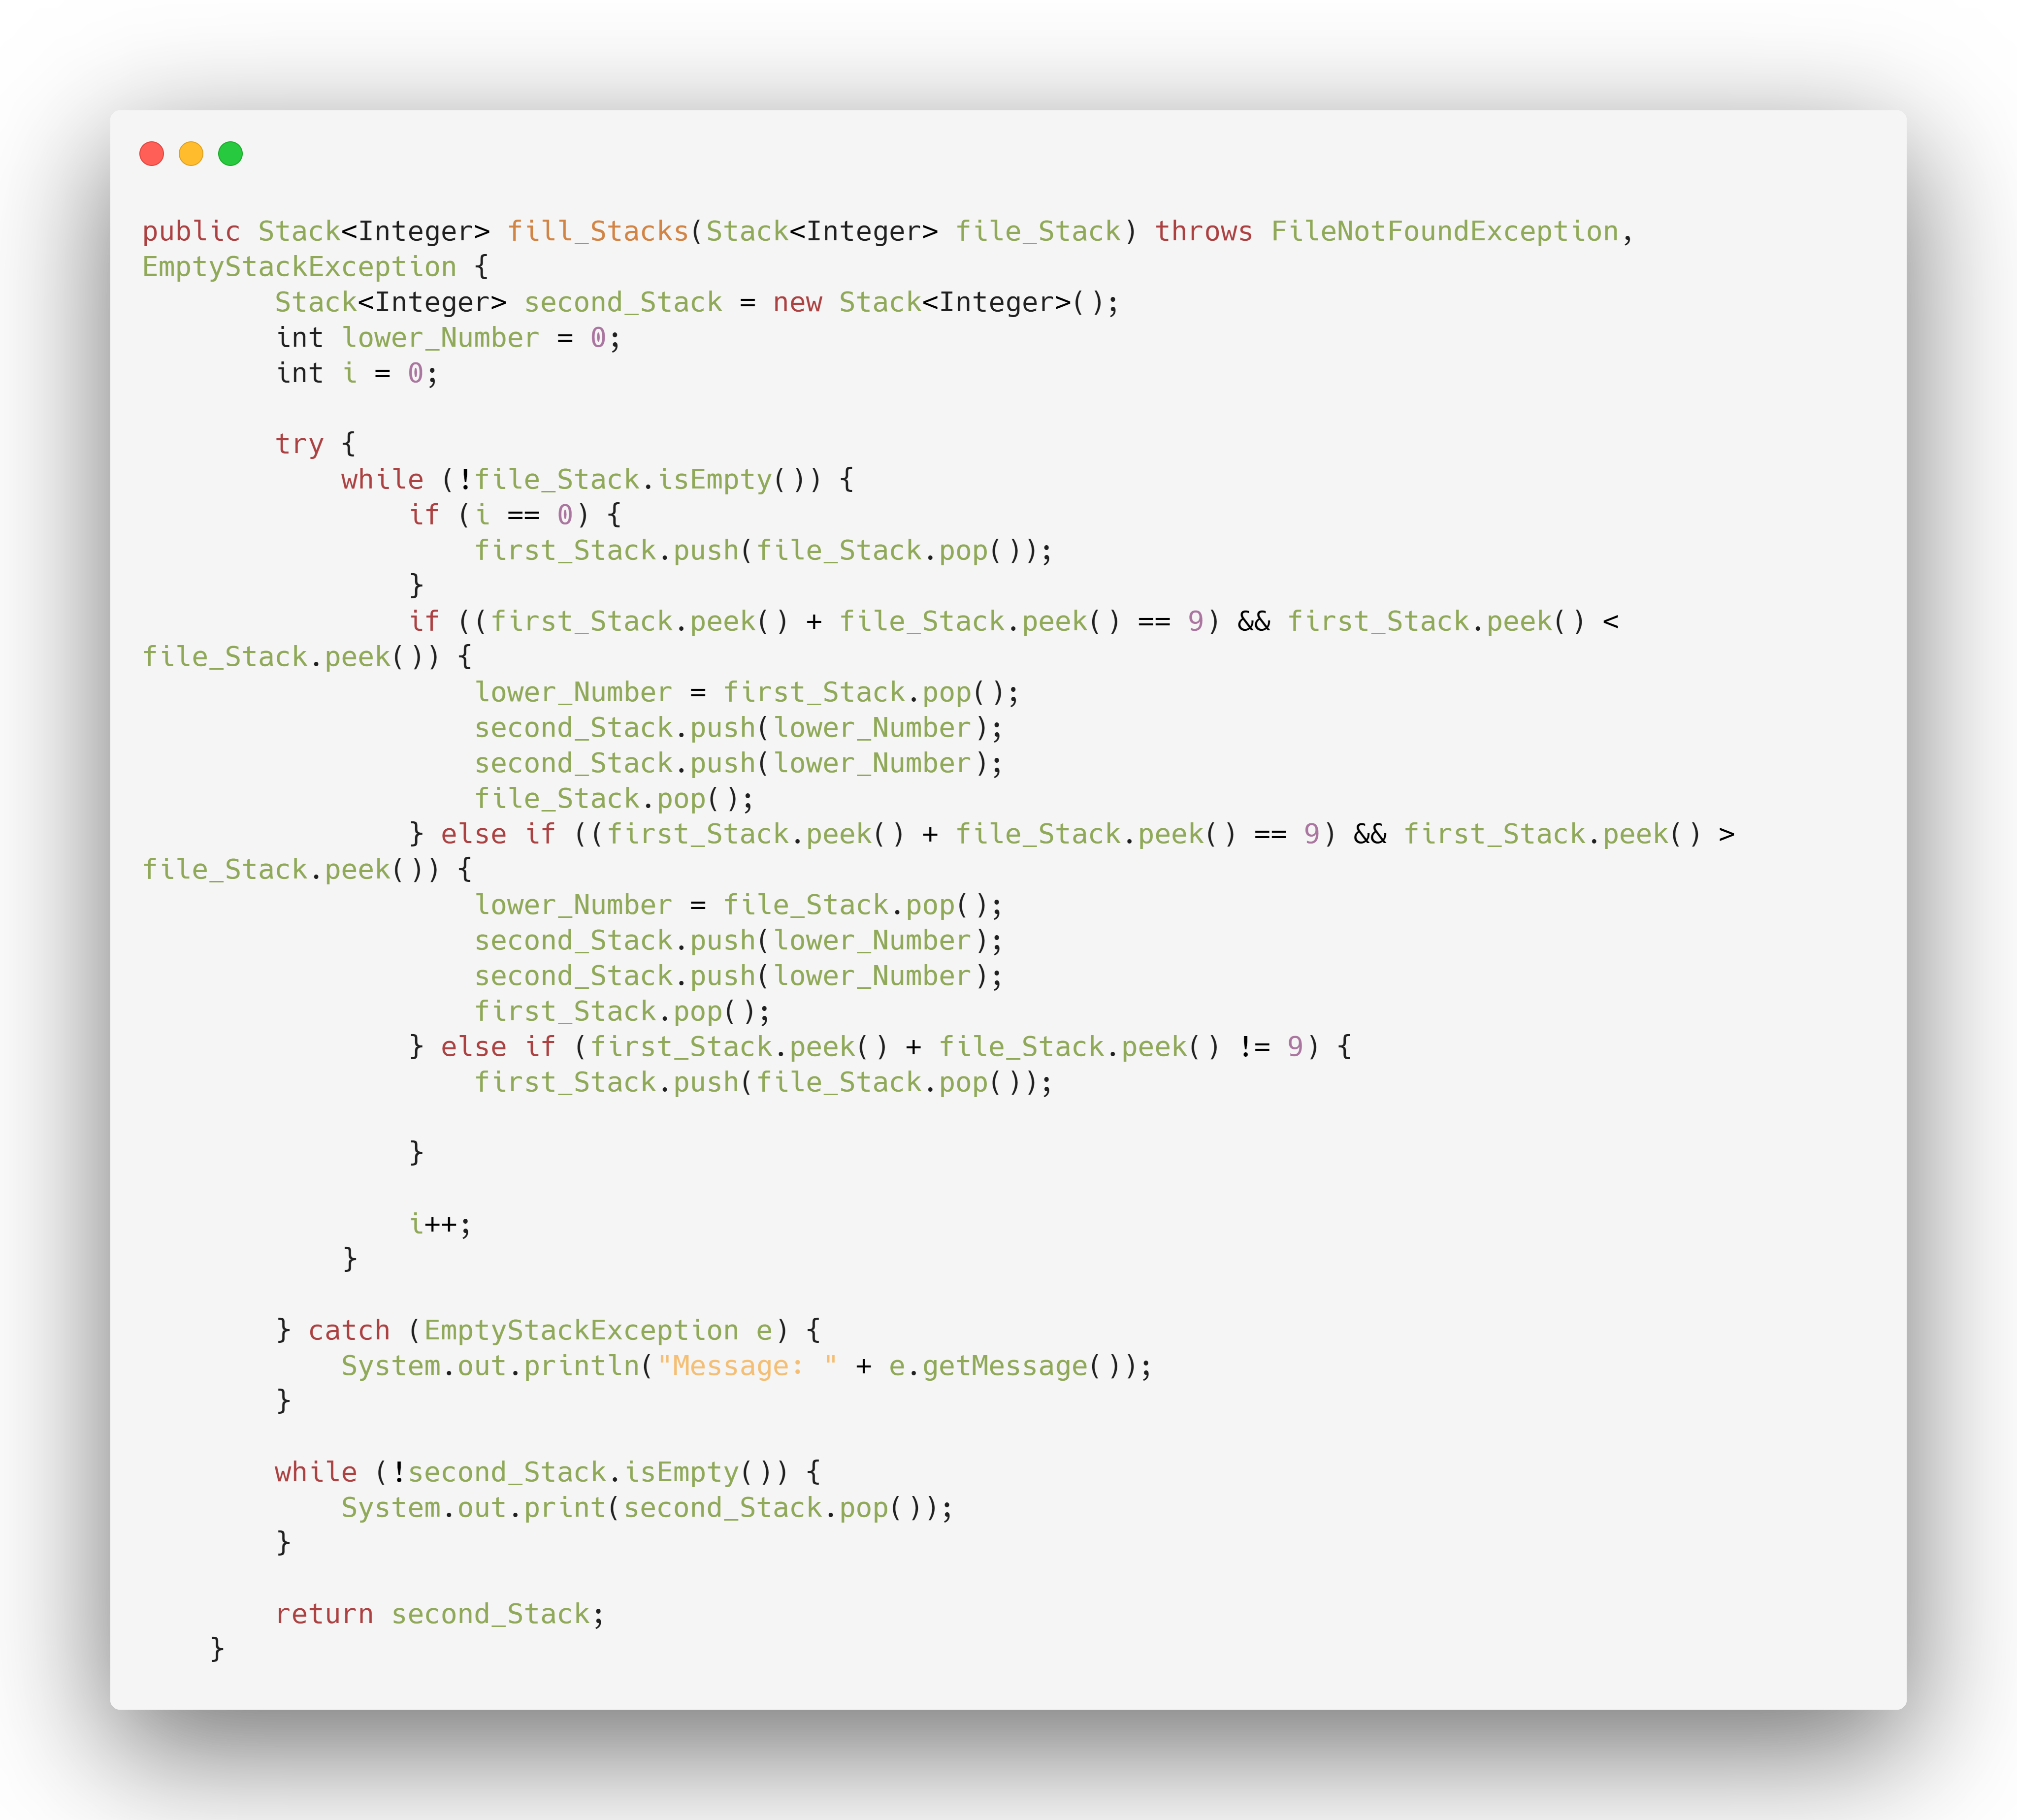
\includegraphics[width=300pt\textwidth]{fill-stack.png}
                     \caption{Code of the fill-stack method}
                     \label{fig:mesh1}
                \end{figure}

\newpage
                \item \textbf{counter-nine}
                This is the second part of the program where the sum of all the numbers in the second-stack is carried out. If the sum between two or more addends is nine or more, a nine is added to the third-stack.
                \begin{figure}[h]
                     \centering
                     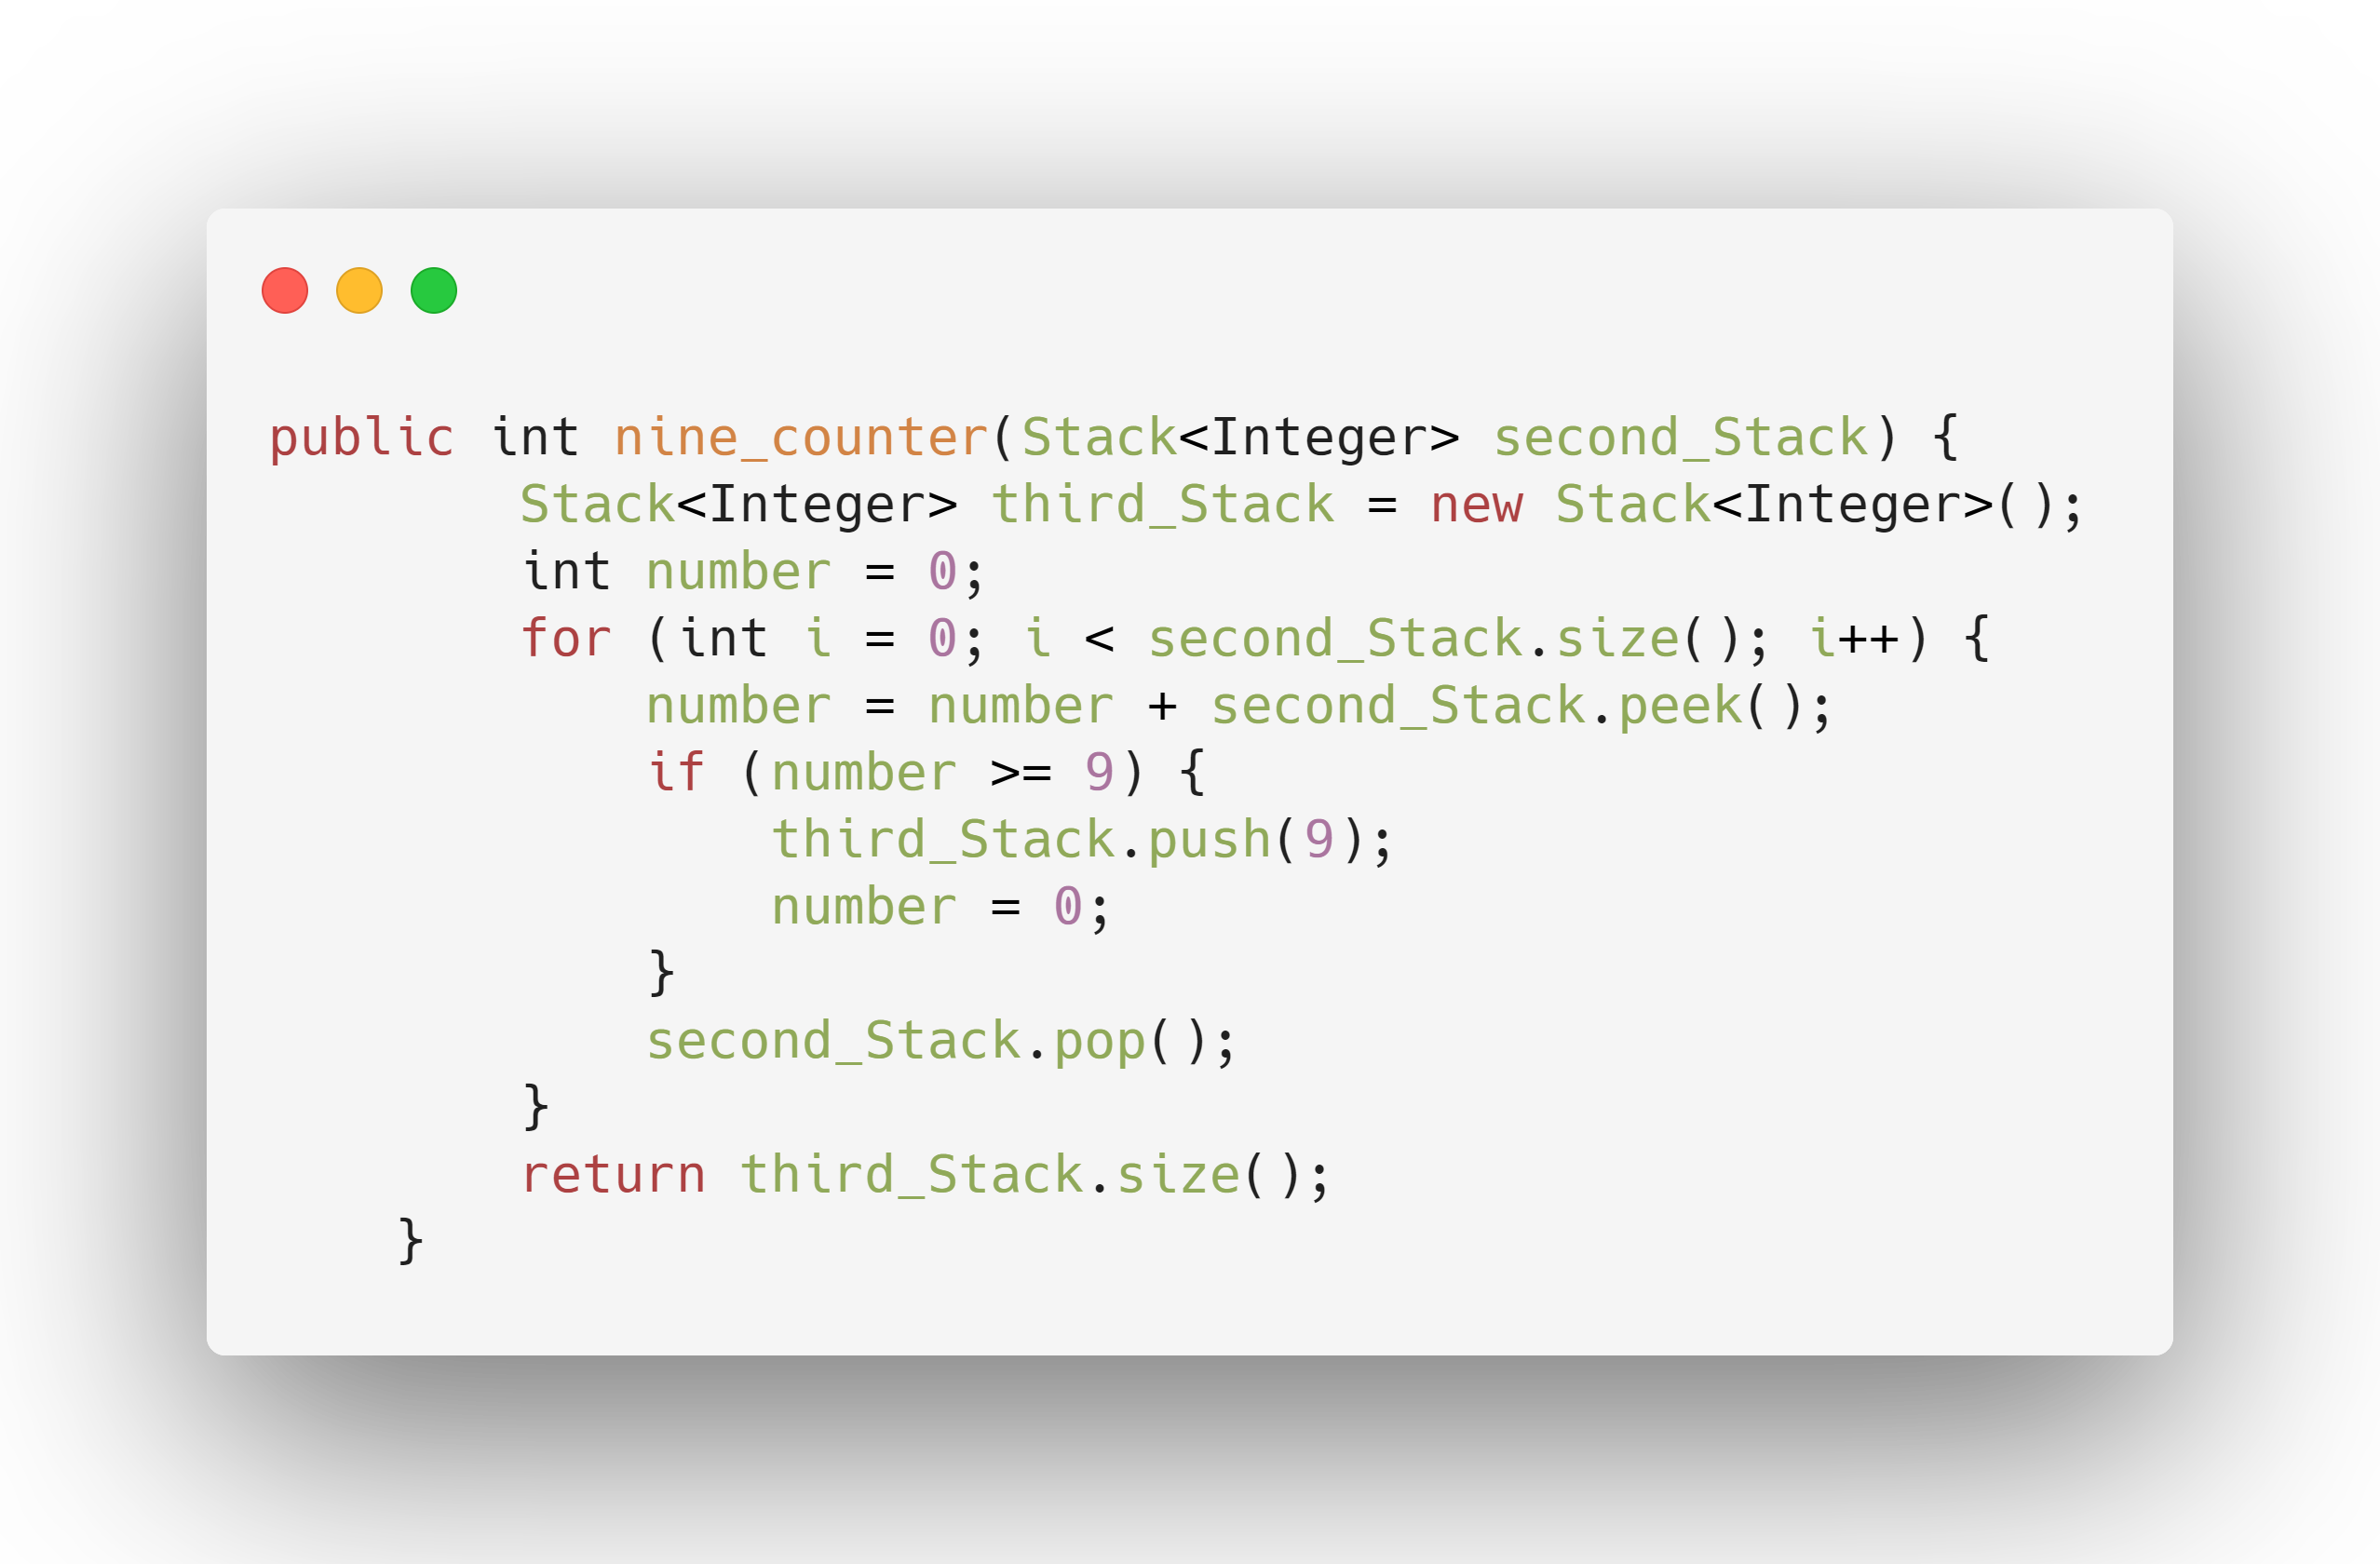
\includegraphics[width=300pt\textwidth]{counter-nine.png}
                     \caption{Code of the nine-counter method}
                     \label{fig:mesh1}
                \end{figure}

                \item \textbf{Problem [constructor]}
                The constructor method is a special method to create and initialise an object created from a class, in our case to create an object of the class "Problem".

            \end{itemize}
        \subsubsection{EmptyStackException}
        This is the custom exception class that we have created. This exception will be thrown when any stack is empty and will prevent the program from crashing.
        \subsubsection{Developing Main class}
        In the main class we have created 3 stacks that, which we will use in the whole problem, then after this we also create and object from the class problem for work with it lately We ask for the direction of the file in your computer (C://naturales.dat.txt) for example, and the Scanner gets the direction of the file.\par When we obtain the direction of it we create a readFile object and with this we invoke the method read form the class readFile and we will obtain the stack with all the numbers. \par
    After this we fill the second stack with the method fill-Stacks from the class Problem.Last of all we take the method nine-counter to count the amount of 9's that we have in the third stack
        \begin{figure}[h]
            \centering
            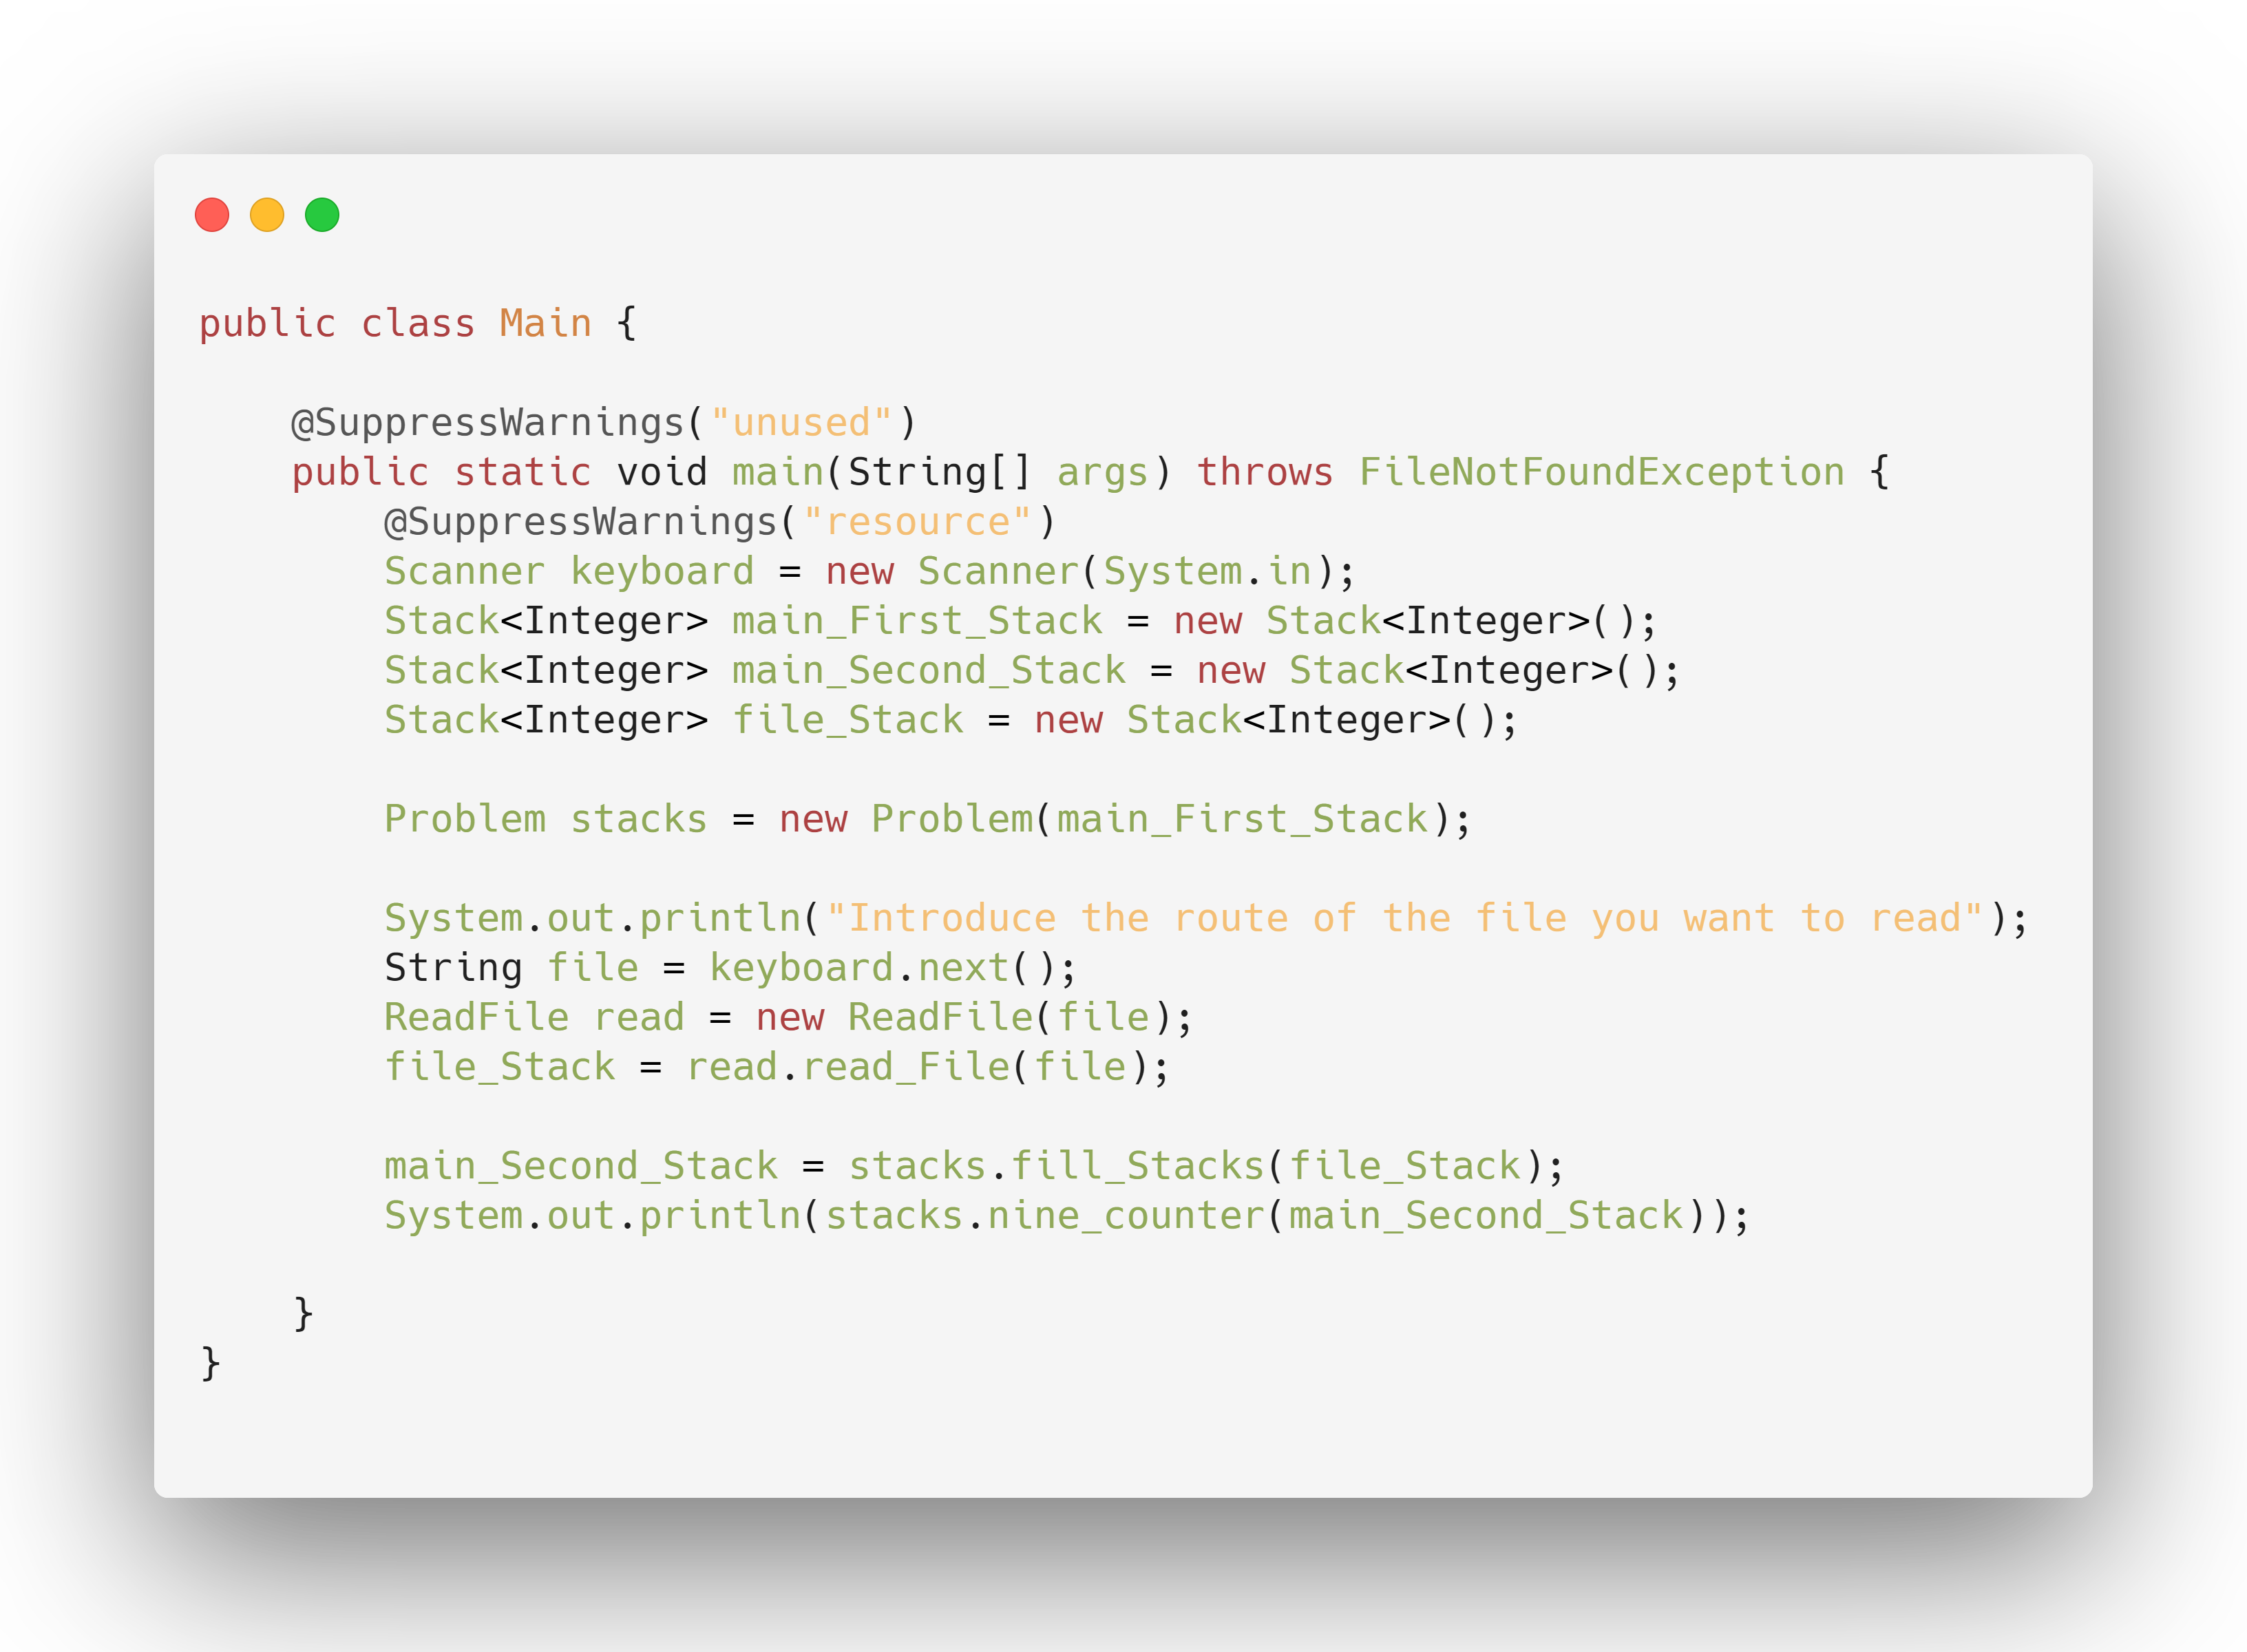
\includegraphics[width=300pt\textwidth]{main-stacks.png}
            \caption{Code of the Main class}
             \label{fig:mesh1}
        \end{figure}
        
        
   \subsection{Technical requirement and running}
        \subsubsection{Generation bat}
        In order to be able to run the programme on an executable we have followed the following steps:
        \begin{itemize}
            \item Create an executable jar of the developed project. 
            \item In a text editor we have written with extension.bat,which we have called Start as if it were the demo of an application.
                \begin{verbatim}

                java -jar nameOfTheJarExecutable.jar
                PAUSE;

                \end{verbatim}
        \end{itemize}
        \subsubsection{Run program}
        To be able to execute this bat the only thing that is needed is to make double click in the file that puts "Start", later, I will ask you the route of the file of which it is wanted to know the number of nines of the third stack.\newline
	
        To run in any IDE it is necessary to follow the following steps:
        \begin{enumerate}
            \item Download and unzip the file containing the code.
            \item Create a project in the IDE of use
            \item Right click on the created project and click on the import option. 
            \item Click on the file system option 
            \item Select the folder with the code to execute
            \item Add the package if necessary in each class
            \item Run the program
        \end{enumerate}
	
	
        
	\newpage
	\section{Queues}
	    \subsection{Problem}
	    A group of friends has decided to organise a music festival. There will be 3 stages in which there will be
        different performances. You need to create a software to manage the festival's capacity. Each stage has its
        own entrance doors, a capacity, and a valid ticket type for the stage. The specifications for each scenario are detailed below:\newline
        \begin{itemize}
            \item Main Stage "Coliseum"
                \begin{itemize}
                    \item Capacity: 25
                    \item Ticket Type: "Platinum"
                    \item Number of entries: 1 (2 optional)
                \end{itemize}
            \item Secondary Scenario "Roar of the Sea"
                \begin{itemize}
                    \item Capacity: 20
                    \item Ticket type: “Platinum”, “Gold”, “SilverSea”
                    \item Number of entries: 1
                \end{itemize}
            \item Third Stage “Siren song”
                \begin{itemize}
                    \item Capacity: 15
                    \item Ticket type: “Platinum”, “Gold”, “SilverSiren”
                    \item Number of entries: 1
                \end{itemize}
        \end{itemize}\newline
        
    The software must simulate the entry of the participants, which will be read from a file called “festival.dat”.
    The result of the program will be the number of people who have entered each stage and the time it has taken
    to fill the capacity. To do this, an average duration has been estimated for each type of ticket:

        \begin{itemize}
            \item Platinum: 2 min
            \item Gold: 3 min
            \item SilverSea: 4 min
            \item SilverSiren: 4 min
        \end{itemize}

	    \subsection{Approach}
    This program allows us to manage and control access to a festival held in a closed recital. To do this, we have had to consider that said venue has different scenarios, which have different access queues. In turn, each of these scenarios has different tickets to access. The program oversees collecting and reading information about the people who are going to enter the venue as well as distributing people between the different queues of the venue to access it, so that it calculates the time they take to enter and the number of people entering each queue. For the program to work, just enter the path of the file that contains the information of the people who are going to enter. Once we enter it, the program will perform the pertinent calculations to return the information described above to the console. \newline

    In order to improve the efficiency of the program, it has been designed in a modular way. From this principle arise the four different classes that make up our program; \textbf{the Readfiles} class, \textbf{the Person} class,\textbf{the Problem } class, and \textbf{the Main}  class. Together they make up the total functionality of our program. 
            \subsubsection{ ReadFile class}
            This class is in charge of reading files. In it, the text data related to the different people is collected, which can be stored in any file on our computer and is read for later organization in the different queues. For this we have in this class a method that is responsible for returning us a queue of text data, which will later be used to create person objects. 
             \subsubsection{ Person class}
            This class helps us to define person objects. It has getters and setters, which provide us with the information related to the two attributes of this class: the name of the stadium and the ticket of the person. 
            \subsubsection{Problem class}
            This class helps us to organise the information we have received from reading the files. In it we have a method to create a new queue of person objects in which are all those people who want to enter, which is generated with the data previously received; with a method to distribute the people in the different rows based on the capacity, the stage they want to access and the type of ticket they have; and, finally, with a method that calculates the time it takes for each of the queues, taking as a reference the types of tickets that each person who wants to access has and is in the queue. 
	        \subsubsection{Main class}
	        This class is the main class. Thanks to it, we control all the aspects that the other classes of our program facilitate us. In it, the reading of files is ordered, then the general queue of people objects is generated, as well as the distribution of people in the different queues. In addition to all this, from this class it is also ordered to print on the console the different times that the queues take as well as the people who have accessed in addition to the total time it has taken to fill the room. 
	     \subsection{Technical requirement and running}
        \subsubsection{Generation bat}
        In order to be able to run the programme on an executable we have followed the following steps:
        \begin{itemize}
            \item Create an executable jar of the developed project. 
            \item In a text editor we have written with extension.bat,which we have called Start as if it were the demo of an application.
                \begin{verbatim}

                java -jar nameOfTheJarExecutable.jar
                PAUSE;

                \end{verbatim}
        \end{itemize}
        \subsubsection{Run program}
        To be able to execute this bat the only thing that is needed is to make double click in the file that puts "Start", later, I will ask you the route of the file of which it is wanted to know the number of nines of the third stack.\newline
	
        To run in any IDE it is necessary to follow the following steps:
        \begin{enumerate}
            \item Download and unzip the file containing the code.
            \item Create a project in the IDE of use
            \item Right click on the created project and click on the import option. 
            \item Click on the file system option 
            \item Select the folder with the code to execute
            \item Add the package if necessary in each class
            \item Run the program
        \end{enumerate}
\newpage
	\section{Lists}
	    \subsection{Problem}
	    The old library of a far away village opened an online platform for books hiring.Now, they want to automatize the process of adding the new books they buy to their catalogue. Using a .txt file with the list of bought books, they want to incorporate them to the system but classified by genre. They have four lists, one for each genre they are specialized in: “Novels”, “Sci-Fi”, “Biographies”, and “Children”. Remember that after adding the new books to the lists, they should be ordered by rating and title if their rating coincide, you can think about extending Comparable Class to make the ordering.\newline
	    
        The Books.txt file contains information about the books they have recently bought in the following format:\newline
            \begin{center}
                Title; Author; Genre; Rating\newline
            \end{center}
    
        Recently, the library owners thought on having a top 10 ranking on their web. So, they also ask for a method that obtains the 3 best rated books from each “adult list” and the best one from the children’s list, and place them on a new list. Also, this list should be ordered by rating.\newline
        
        Finally, for promotion purposes, pick the last book in the top 10 list, set it the highest rating (5 stars), and place
        it the first in the list, then, increment in 0.5 all the ratings of this list using \textbf{replaceAll()} method.\par
        
        The program should give as a result the 5 lists ordered by rating and title.\par

    \subsection{Approach}
	    The main idea to develop this project is to divide it into classes according to each of the functions. That is why, we have created a \textbf{ReadFile} class which is in charge of reading the file provided to us for the practice, the \textbf{Problem} class where most of the code will be developed solving the problem ,the \textbf{Book} class where we will develop the objects for each book in the file, The \textbf{UnitaryOperator} class which content the method replaceAll() and the \textbf{Main} class where only calls to methods of the classes will be made and the result will be shown by console. All this by means of an object oriented programming.
	    
	    
	    
	    \subsubsection{ ReadFile class}
	    The main function of this class is to read the file containing the information of the books in the library. \newline

        The approach is that as the books are separated by ";", divide with the string tokenizer where each field will be stored in the variables tittle, author, genre and rating and these variables will be put together to create the objects books. One object for each book in the file.\newline

        After dividing each of the sections and creating the book object, we add them to the list called list-book-file.
        
        As a note when creating the book objects, the rating attribute must be parsed because the String tokenizer only reads strings and this attribute is a double.
        
        This class also contains a method called ReadFile which is the constructor of the class.
    
	    \subsubsection{ Book class}
	    
	    The book class will be in charge of creating the objects with the following attributes: title, author, genre and punctuation.\newline

         This class also contains each of the getters and setters corresponding to each attribute in order to access the information of the object and/or modify it, respectively.\newline

         It has a method called toString() that we make use of it when we need to print the information of each object, its format is the following:\newline
    
            \begin{verbatim}
            public String toString() {
                return "Author=" + author + "\nTittle=" + tittle + "\nGenre=" + 
                genre + "\nrating=" + rating +"\n"
            }
             \end{verbatim}
        \begin{itemize}    
            \item\textbf{compareTo() method}\newline
                As we have to order the lists according to the score they have and if they coincide in this by the title of the book, we have decided to make this method according to the result which returns. The idea is that the object of book that there is in a list meets any of the following rules when compared to the book object passed as an argument, they will be sorted according to what they return.We are comparing the rating between the objects. Rules: \newline
                
                \begin{itemize}
                    \item if( rating book a lower than rating book b) return 1.Book b has a greater rating.
                    \item if( rating book a greater than rating book b) return -1.Book a has a greater rating.
                    \item if( rating book a == rating book b), both books have the same rate son we will compare between their title (the first letter). \par
                    
                    For the comparison between titles we add the two to compare in an array and we order them, then we check with the same conditions as with the rating which one is higher or lower. \par  
                    
                    For example, in the first if if the psoicon zero of the array is greater than the one being compared a minus one is returned which implies that it is a title that goes before the one being compared.
                \end{itemize}
                This method is used by the implementation of the class comparable.
          \end{itemize}


	    \subsubsection{Problem class}
	    This class will contain all the methods that will be needed to develop the list project, with the idea of only having to call them in the main.
	    
	    \begin{itemize}
	        \item \textbf{Problem()}\newline
	         The constructor method is a special method to create and initialise an object created from a class, in our case to create an object of the class "Problem".
	        \item \textbf{fill-stacks() method} \newline
	          The idea of this method is to read the list containing the books read from the file and classify them according to their genre when called in the main.\newline

                If the list is empty it adds it directly, if it is not, it will check if it is not in the list and if it is, it will not operate with it. But if it is not, we call the \textbf{compareTo()} method to classify them by rating and title if the rating is the same.


	        \item \textbf{top-ten() method }\newline
	        It consists of creating a top ten of the books in the bookshop with three of each of the adult genres and one for children.\newline

            The idea is to go through the adult lists up to position three and add them to the top ten list, while the list of children's books will only take the first one.\newline

            To order them we follow the same approach as in previous methods.
	        \item \textbf{top-ten-promo() method }\newline
	        The curiosity of this method is that we go through the top ten list but we don't edit directly on it because when we make any modification we modify all the created lists.\newline

            To solve this problem we have gone through the list and recreated each object in that list and added it to another one so as not to have any unnecessary modification.\newline

            We moved the last book in the list and put it in the first one modifying its rating.\newline

            Then we call the \textbf{replaceAll()} method where we change the value of all rating.\newline


	        
	    \end{itemize}
	    
	    
	    
	    
	    
	    
	    
	    
	    
	    
	    
	    
	    
	    
	    \subsubsection{UnitaryOperator class}
	        We implement this class as described in the practice statement where it will contain the replaceAll() method.
    \begin{itemize}
    \item \textbf{replaceAll() method}\newline
    The idea of this method is to pass a book as argument to obtain the score of that book and to modify it adding 0.5. It will return the book with the replaced score when the method is called.
     \begin{verbatim}
     
     class Uo implements UnaryOperator<Book> {
         public Book apply(Book book_to_replace) {
             book_to_replace.setRating(book_to_replace.getRating()+0.5);
      return book_to_replace;
         }
    }
     \end{verbatim}
\end{itemize}



	    \subsubsection{Main class}
	    For the visual operation of the lists program we have decided to represent it by means of a menu where each option will show one of the lists requested by the statement.\newline

        The idea of the menu is the following:\par
        \begin{enumerate}
            \item Novel books
            \item Sci-fi books
            \item Biography books
            \item Children books
            \item Top 10 books
            \item Top 10 books in promo
            \item Exit
        \end{enumerate}
    Although the programme should only show five lists, we have included a last option showing the list that is modified when we add 0.5 to the score of the books, with the idea of showing that it also worked.
    
    \subsection{Technical requirements}
        \subsubsection{Generation bat}
            In order to be able to run the programme on an executable we have followed the following steps:
        \begin{itemize}
            \item Create an executable jar of the developed project. 
            \item In a text editor we have written with extension.bat,which we have called Start as if it were the demo of an application.
                \begin{verbatim}

                java -jar nameOfTheJarExecutable.jar
                PAUSE;

                \end{verbatim}
        \end{itemize}
        \subsubsection{Run program}
	     To be able to execute this bat the only thing that is needed is to make double click in the file that puts "Start", later, I will ask you the route of the file of which will show a menu where the user could select which ranking list it want to watch, if the user want close the program he will select the last option of the menu.\newline
	
        To run in any IDE it is necessary to follow the following steps:
        \begin{enumerate}
            \item Download and unzip the file containing the code.
            \item Create a project in the IDE of use
            \item Right click on the created project and click on the import option. 
            \item Click on the file system option 
            \item Select the folder with the code to execute
            \item Add the package if necessary in each class
            \item Run the program
        \end{enumerate}
        

        
        
	
%	\newpage

	
	
\end{document}